\documentclass[a4paper,11pt]{article}
\usepackage[a4paper, left=1.5cm, right=1.5cm, top=2.0cm, bottom=3.5cm, headsep=1.2cm]{geometry}
\usepackage{polski}
\usepackage{amssymb}
\usepackage[utf8]{inputenc}
\prefixing
\usepackage{latexsym}
\usepackage{graphicx}
\usepackage{hyperref}
\author{Klaudia Balcer}
\title{Regresja Poissona}
\frenchspacing
\begin{document}
\maketitle
\begin{center}
Zaawansowane Modele Liniowe

Raport 3 
\end{center}
\tableofcontents

\section*{Wstęp}

Poniższy raport bazuje na danych \textit{sklep} zawierających w kolumnach dane dotyczące dnia tygodnia, godziny, liczby klientów w sklepie i zmienna binarną informującą o wydarzeniach sportowych danego dnia. W nieniejszym raporcie, za pomocą regresji Poissona przeanalizuję te dane,  wybierając optymalny model. Pracę rozpocznę od wizualizacji danych. Spostrzeżenia sprawdzę badając właściwości kolejnych modeli. Uzyskawszy optymalny sposób predykcji podam wyniki konfrontując je  ponownie z danymi i zaproponuję grafik z uwzględnieniem wyników oraz prawa pracy. 



\pagebreak

\section{Wizualizacja danych}



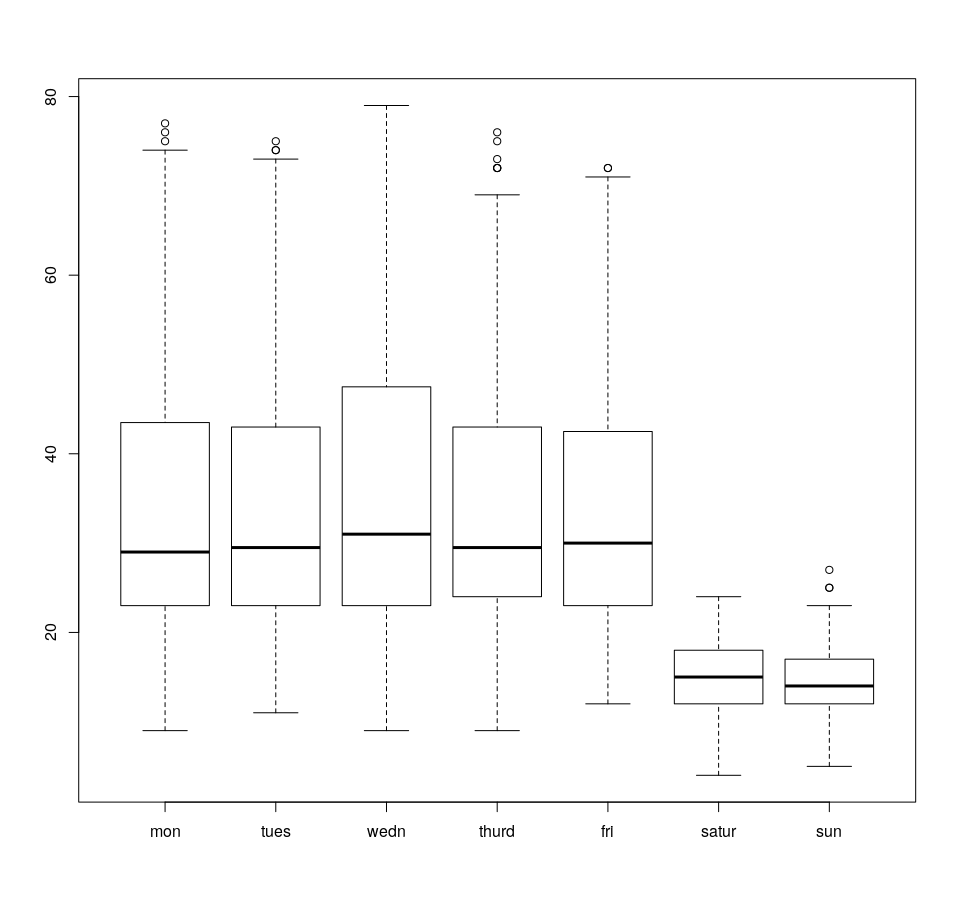
\includegraphics[scale=.7]{boxplot1.png} 

Widzimy, że w weekend ilość klientów jest wyraźnie mniejsza niż w dni robocze. Ponadto rozstrzał między ilością klientów  w dni weekendowe jest znacznie mniejszy niż w dni robocze. Warto też zauważyć, że w dni robocze ilość klientów w kolejnych godzinach ma niesymetryczny rozkład. 

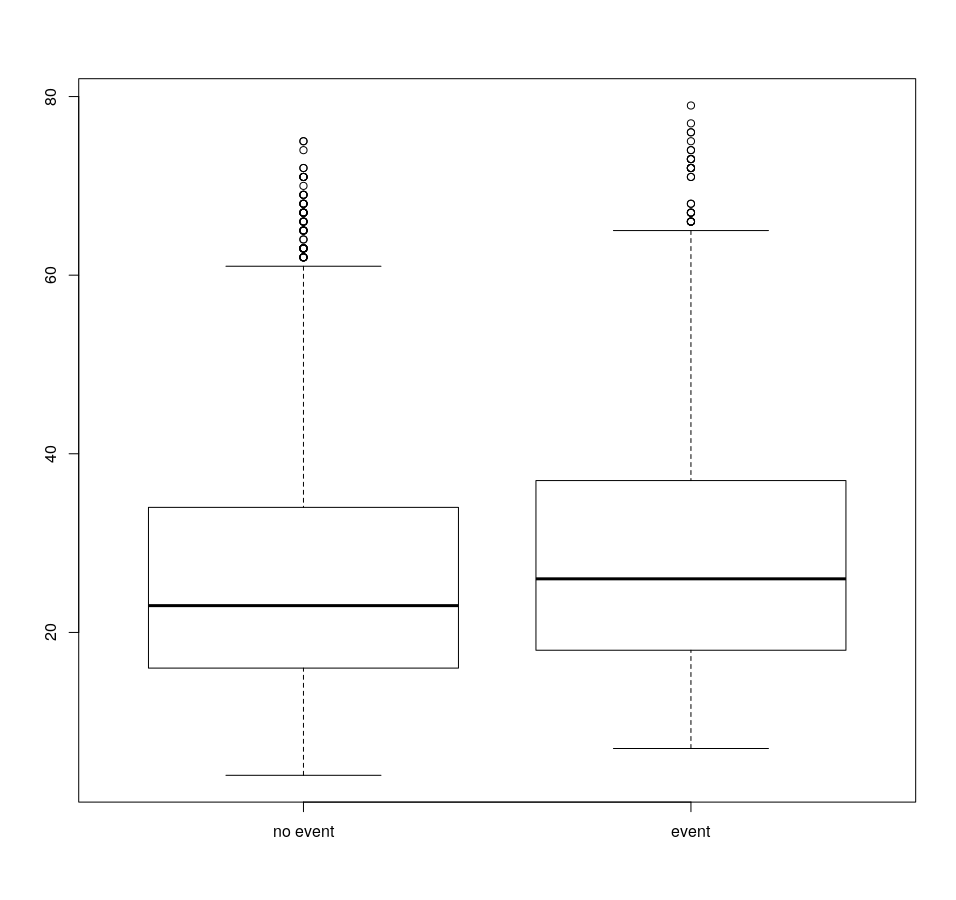
\includegraphics[scale=.7]{boxplot2.png} 

Różnica między ilościami klientów w dniach wydarzeń sportowych różni się nieznacznie od dni bez takich imprez. Rozkłady te są dość podobne, wykazują niewielką asymetrię i małą różnicę w medianie.

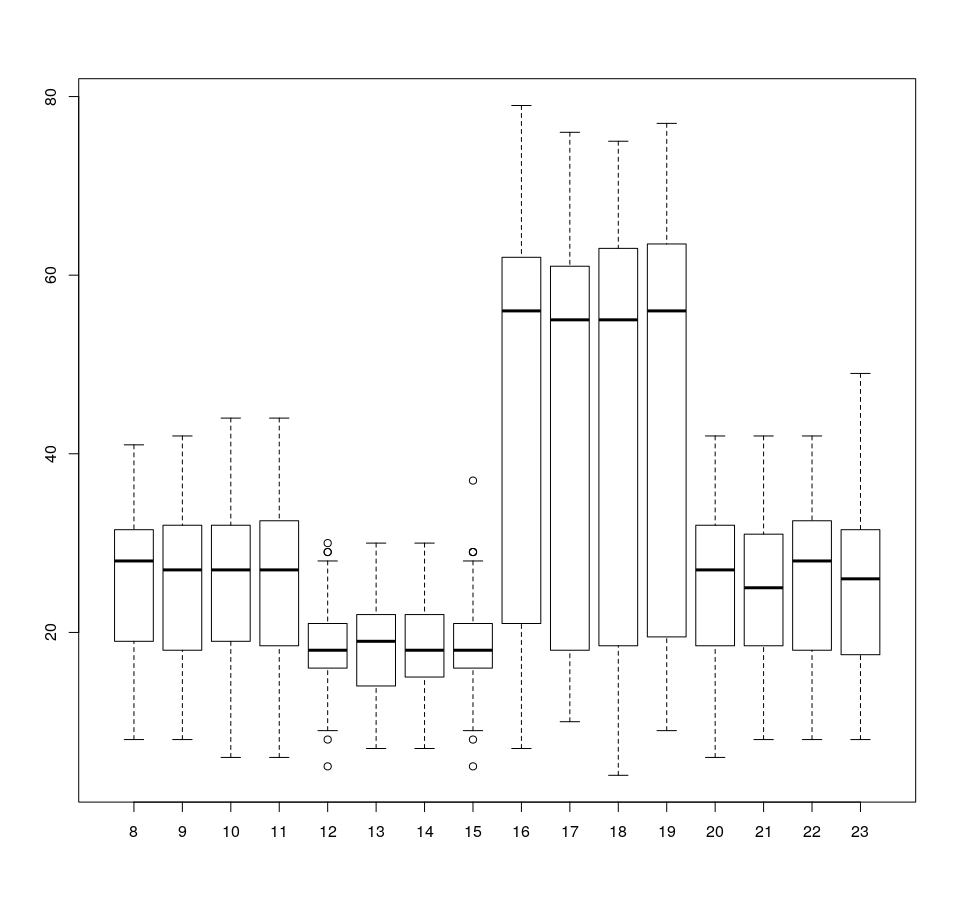
\includegraphics[scale=.7]{boxplot3.png} 

Między 12 a 16 wariancja ilości klientów w kolejnych dniach jest wyraźnie mniejsza niż o innych porach. Największe wahania wysętpuję w godzinach poppołudniowych - od 16 do 20. Tam w zależności od dnia ilości klientów są bardzo różne, ponadto rozkład liczby osób korzystających ze sklepu jest wyraźnie niesymetryczny - zdecydowanie więcej jest\textit{dużych} obserwacji. 

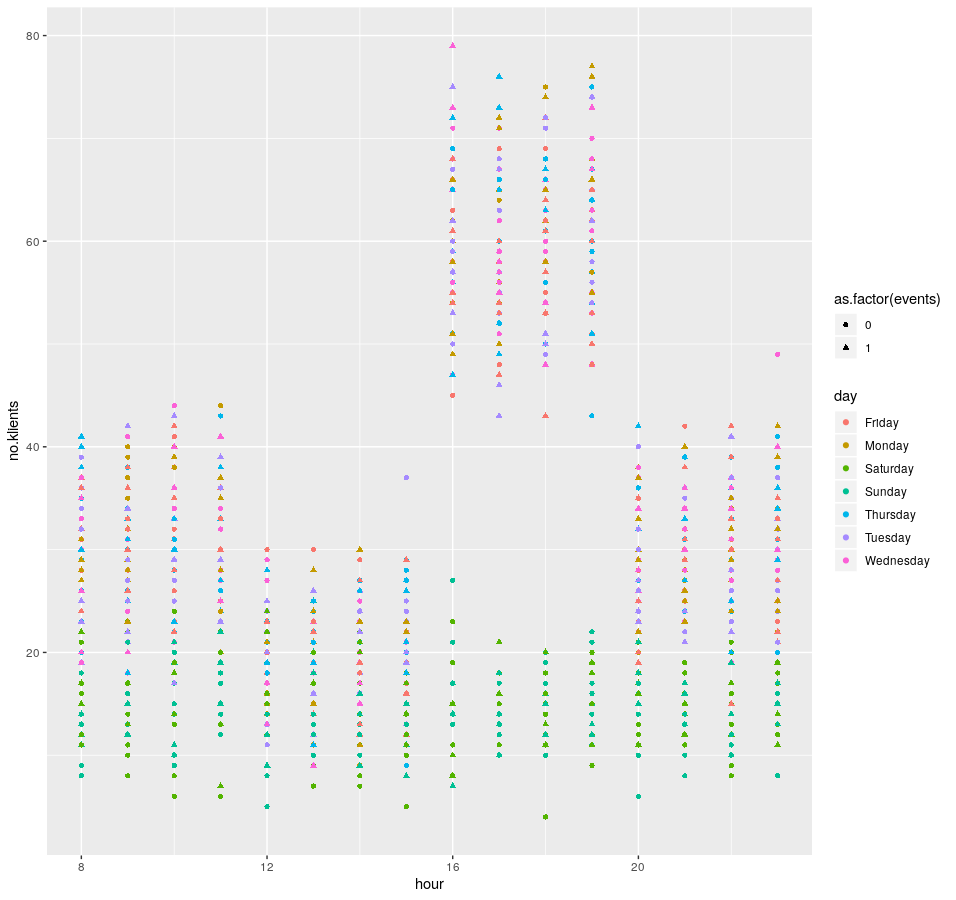
\includegraphics[scale=.7]{plot1.png} 

Obserwacje zależnie od występowania wydarzeń sportowych są podobne. W soboty i niedziele klientów jest mniej niż w pozostałe dni. Szczególnie dobrze widać to w godzinach popołudniowych 16-20.  Ilość klientów w dni robocze jest o tej porze znacznie wyższa niż o pozostałych w dni robocze, natomiast w weekendy  utrzymuje się na podobnym poziomie co w inne dni. 

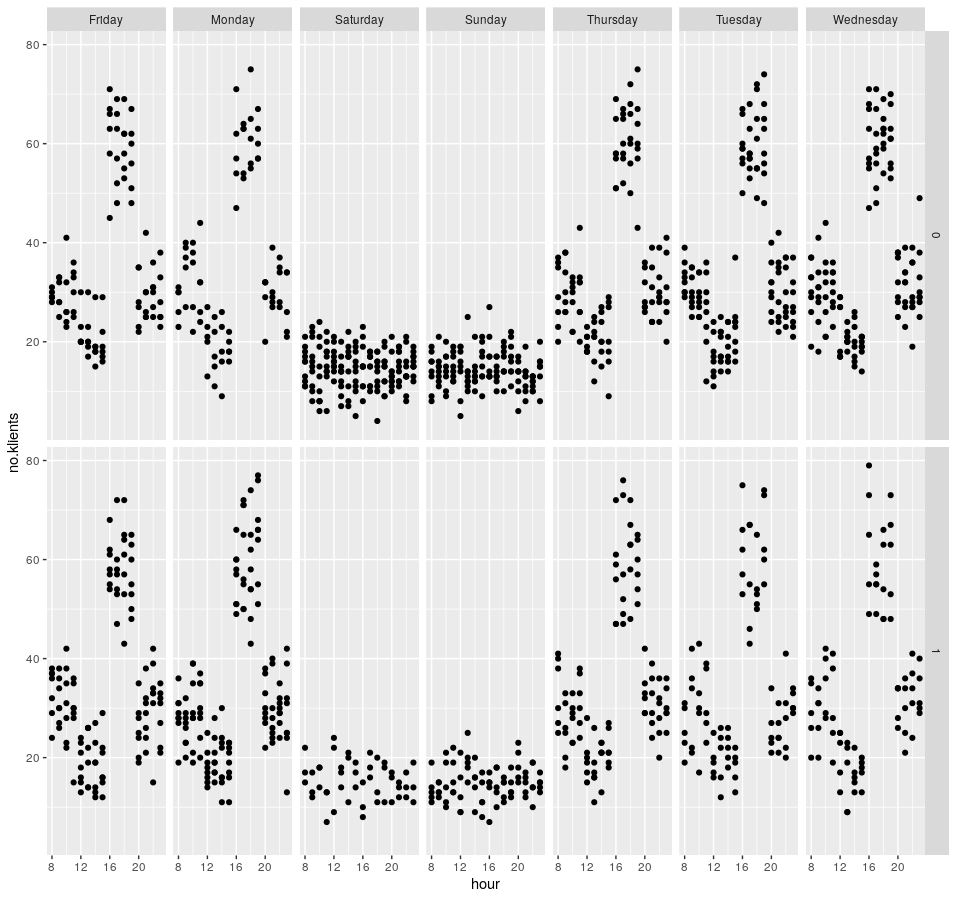
\includegraphics[scale=.7]{plot2.png} 

Bez względu na wydarzenia sportowe różnice w rozkładzie ilości klientów na godzinę zależą wyłącznie od dnia tygodnia. Możemy też zauważyć, że obserwacji z dni z imprezami jest mniej. Co  mogłoby być przyczyną drobnych różnic w rozkładach ilości klientów w zależności od imprez sprotowych.

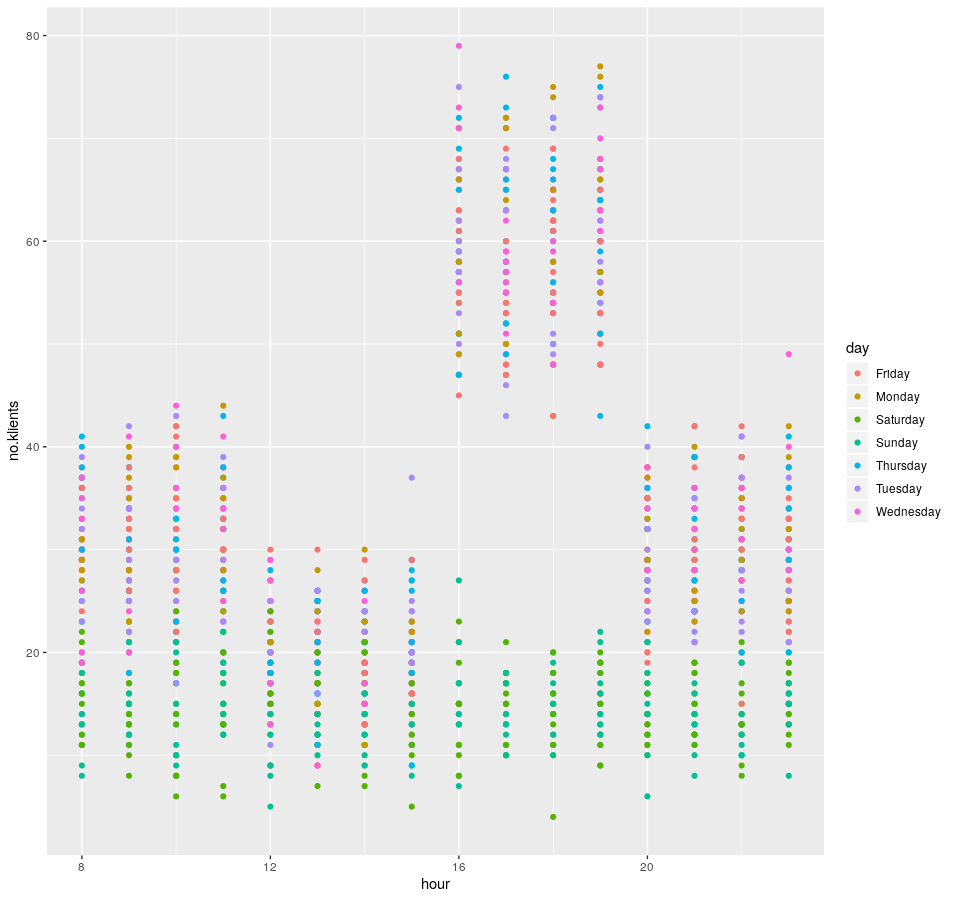
\includegraphics[scale=.7]{plot3.png} 

Powyższy i kolejny wykres są analogiczne do  dwóch poprzednich, niemniej nie obejmują już podziału na dni z i bez wydarzeń sportowych. 

Widzimy powody asymetrii na boxplotach. W boxplotach dla godzin 16,  17, 18,  19 rozstrzał był tak duży, bo inaczej wygląda ruch w dni robocze i weekendowe. W boxplotach dla dni roboczych rozstrzał natomiast powodowany był różnicami w zależności od pory dnia. 

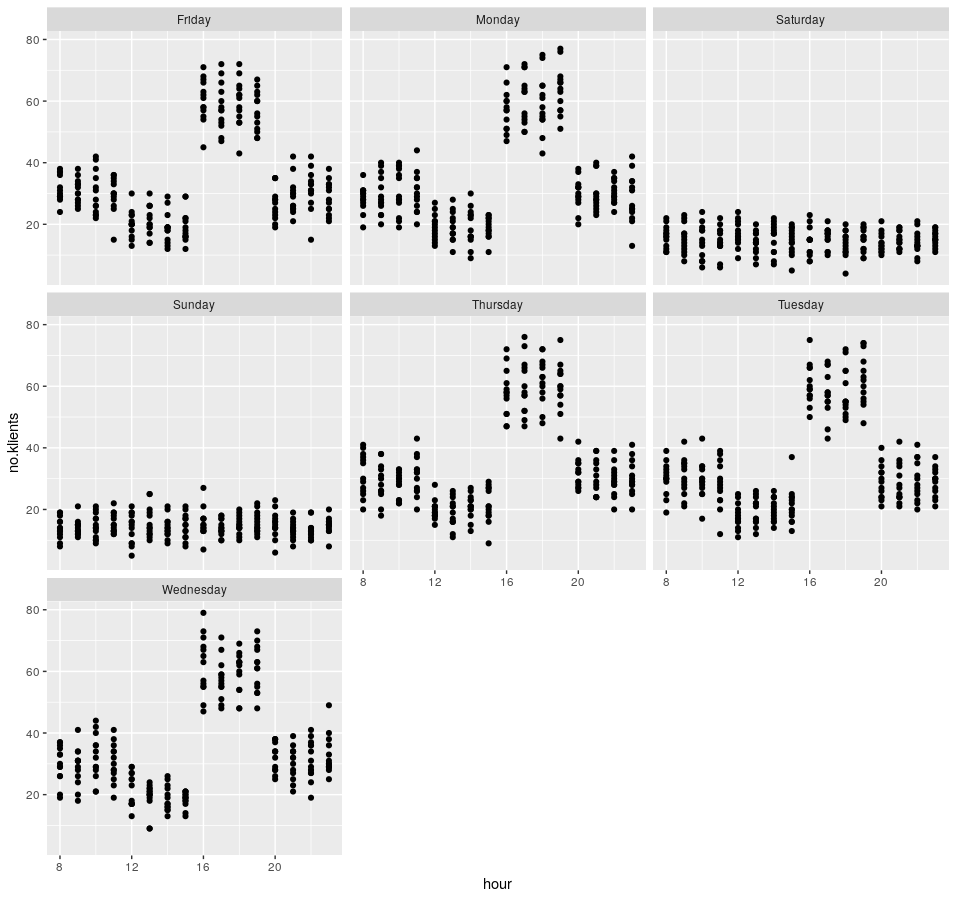
\includegraphics[scale=.7]{plot4.png} 

W weekendy liczba klientów wydaje się spoczywać na podobnym poziomie przez cały dzień. W tygodniu podobieństwa obserwujemy w czterogodzinnych blokach. O różnych porach dnia ilości klientów różnią się znacznie - z szczególnym skokiem od 16 do 20.

Patrząc na wszystkie wykresy możemy się spodziewać, że nie wszystkie zmienne będą istotne. Ponadto być może podział na bloki godzinowe czterogodzinne i podział dni tylko na robocze i weekendowe może dać nam lepszy model. Zasadnym wydaje się również wykorzystanie modelu z interakcją między porą dnia a tym, czy dzień jest roboczy.

Sprawdźmy czy testy na modelach, które można zbudować na podstawie danych i tych przesłanek, faktycznie potwierdzają zasadność takiej redukcji. 



\section{Pełny model}

\subsection{Model ze wszystkimi podanymi zmiennymi, bez interakcji}

Jako pierwszy przedstawię model, po który pewnie sięgnęlibyśmy bez wcześniejszej wstępnej analizy i wizualizacji danych. Model z wykorzystaniem wszystkich zmiennych objaśniających, które nam podano, bez interakcji, z faktorami wynikającymi wprost z danych.

\paragraph{Fragment summary modelu}

\begin{verbatim}
Call:
glm(formula = no.klients ~ day + factor(hour) + factor(events), 
    family = poisson, data = sklep)

Deviance Residuals: 
    Min       1Q   Median       3Q      Max  
-5.0561  -0.8943  -0.0331   0.8217   4.3186  

Coefficients:
                 Estimate Std. Error z value Pr(>|z|)    
(Intercept)      3.431727   0.023847 143.905   <2e-16 ***
dayMonday        0.005199   0.016684   0.312    0.755    
daySaturday     -0.846422   0.021723 -38.964   <2e-16 ***
daySunday       -0.861595   0.021688 -39.726   <2e-16 ***
dayThursday      0.014026   0.016640   0.843    0.399    
dayTuesday      -0.003875   0.016763  -0.231    0.817    
dayWednesday     0.022958   0.016653   1.379    0.168    
factor(hour)9   -0.016261   0.029255  -0.556    0.578    
factor(hour)10  -0.011097   0.029217  -0.380    0.704    
factor(hour)11  -0.008525   0.029198  -0.292    0.770    
factor(hour)12  -0.334606   0.031899 -10.489   <2e-16 ***
factor(hour)13  -0.347741   0.032022 -10.859   <2e-16 ***
factor(hour)14  -0.351353   0.032056 -10.961   <2e-16 ***
factor(hour)15  -0.342945   0.031977 -10.725   <2e-16 ***
factor(hour)16   0.592304   0.025675  23.070   <2e-16 ***
factor(hour)17   0.579071   0.025736  22.501   <2e-16 ***
factor(hour)18   0.590189   0.025684  22.979   <2e-16 ***
factor(hour)19   0.610448   0.025592  23.853   <2e-16 ***
factor(hour)20  -0.012385   0.029226  -0.424    0.672    
factor(hour)21  -0.024926   0.029319  -0.850    0.395    
factor(hour)22  -0.009810   0.029208  -0.336    0.737    
factor(hour)23  -0.010239   0.029211  -0.351    0.726    
factor(events)1 -0.011612   0.009998  -1.161    0.245    
\end{verbatim}

Itercept pokazuje ilość klientów w piątek o 8 rano. Widzimy, że istotne zmiany ze względu na dzień zaobserwować można tylko w sobotę i niedzielę. Istotne zmiany po wzięciu pod uwagę pory dnia widzimy od 12 do 16 kiedy klientów jest mniej (współczynniki dla kolejnych czynników mają w tym przedziale podobne wartości oscylujące wokół -0.34) oraz od 16 do 20 gdzie klientów jest więcej (współczynniki również mają podobne wartości - około 0.59). O pozostałych porach sytuacja jest podobna jak w pierwszej godzinie działania sklepu. Wydarzenia sportowe nie jawią się jako istotny czynnik. 

Model  ten z jednej strony sugeruje wykowanie redukcji, z drugiej zaś  brakuje w nim interakcji, którą widzieliśmy w graficznej interpretacji danych. Inaczej wygląda sprawa w piątek o 17 niż w sobotę  o 17. Tak więc przed dokonaniem redukcji sprawdźmy jak w takim razie będzie się przezentował modoel z interakcją. 

\subsection{Model ze wszystkimi podanymi zmiennymi, z interakcją}

\paragraph{Obserwacje}

Model ten składa się z 223 zmiennych objaśniających. Jendak raptem 33 są istotne, ww tym 23 interakcje (głównie dni weekendowe:godziny popołudniowe, kilka interakcji wtorek,niedziala:godzina:event). Model uwzględnia zmienną event i 111 interakcji nią, z czego tylko 9 jest istotnych. Potwierdza się jednak interakcja między popołudniowymi godzinami z sobotami i niedzielami Pokażę fragment summary, wybierając jedynie istotne $X_{i}$.  

\paragraph{Frahment summary}

\begin{verbatim}
Call:
glm(formula = no.klients ~ day * factor(hour) * factor(events), 
    family = poisson, data = sklep)

Deviance Residuals: 
    Min       1Q   Median       3Q      Max  
-3.4245  -0.6890  -0.0545   0.6201   2.6813  

Coefficients:
                                            Estimate Std. Error   z value     Pr(>|z|)
(Intercept)                                3.3787245 0.07537784 44.823846 0.000000e+00
daySaturday                               -0.6443570 0.11034185 -5.839643 5.231283e-09
daySunday                                 -0.7307782 0.12054615 -6.062228 1.342486e-09
factor(hour)12                            -0.2801349 0.11489393 -2.438204 1.476043e-02
factor(hour)13                            -0.3106716 0.11590408 -2.680420 7.352989e-03
factor(hour)14                            -0.3997994 0.11898065 -3.360205 7.788464e-04
factor(hour)15                            -0.3746934 0.11809437 -3.172831 1.509605e-03
factor(hour)16                             0.7430190 0.09156703  8.114482 4.878614e-16
factor(hour)17                             0.7016338 0.09218850  7.610860 2.722775e-14
factor(hour)18                             0.7128384 0.09201812  7.746718 9.429801e-15
factor(hour)19                             0.6701577 0.09267575  7.231208 4.787155e-13
daySaturday:factor(hour)12                 0.3430487 0.16059789  2.136072 3.267353e-02
dayTuesday:factor(hour)12                 -0.3867444 0.15623797 -2.475355 1.331039e-02
daySaturday:factor(hour)14                 0.3734821 0.16527723  2.259731 2.383795e-02
daySunday:factor(hour)14                   0.3728919 0.17915596  2.081382 3.739899e-02
daySunday:factor(hour)15                   0.4835875 0.17530643  2.758527 5.806248e-03
daySaturday:factor(hour)16                -0.7495337 0.14633514 -5.122035 3.022558e-07
daySunday:factor(hour)16                  -0.5651321 0.15697606 -3.600116 3.180750e-04
daySaturday:factor(hour)17                -0.7346401 0.14732154 -4.986644 6.143704e-07
daySunday:factor(hour)17                  -0.7194914 0.16234927 -4.431750 9.347122e-06
daySaturday:factor(hour)18                -0.8519512 0.14974485 -5.689352 1.275221e-08
daySunday:factor(hour)18                  -0.6039443 0.15891317 -3.800467 1.444235e-04
daySaturday:factor(hour)19                -0.7442656 0.14857761 -5.009272 5.463640e-07
daySunday:factor(hour)19                  -0.4997057 0.15780062 -3.166690 1.541845e-03
dayTuesday:factor(events)1                -0.3765239 0.14693007 -2.562606 1.038898e-02
dayTuesday:factor(hour)11:factor(events)1  0.6099298 0.20771201  2.936420 3.320241e-03
dayTuesday:factor(hour)12:factor(events)1  0.6929291 0.23348712  2.967740 2.999978e-03
daySunday:factor(hour)13:factor(events)1   0.5083964 0.25920825  1.961343 4.983898e-02
dayTuesday:factor(hour)14:factor(events)1  0.6103763 0.23162569  2.635184 8.409170e-03
dayTuesday:factor(hour)16:factor(events)1  0.4708986 0.17890047  2.632182 8.483843e-03
dayTuesday:factor(hour)17:factor(events)1  0.3558529 0.18063341  1.970028 4.883513e-02
dayTuesday:factor(hour)19:factor(events)1  0.4595039 0.17938095  2.561609 1.041885e-02
daySunday:factor(hour)20:factor(events)1   0.6145479 0.25537287  2.406473 1.610741e-02
dayTuesday:factor(hour)23:factor(events)1  0.5010963 0.20816636  2.407191 1.607575e-02

(Dispersion parameter for poisson family taken to be 1)

    Null deviance: 12434.9  on 1455  degrees of freedom
Residual deviance:  1359.6  on 1232  degrees of freedom
AIC: 9185.5

Number of Fisher Scoring iterations: 4

\end{verbatim}

\paragraph{Wniosek:}

Model ten zdecydowanie wymaga redukcji. 

Bazując na graficznej interpretacji danych proponuję podział dni na robocze i weekendowe oraz ułożenie czterogodzinnych bloków w ciągu dnia. W takich grupach obserwowaliśmy analogie. 

\section{Zredukowany model regresji Poissona}

Budując nowe zmienne czynnikowe nazwałam faktory nie jako kolejne liczby naturalne,  ale  jako teksty. Zmienne czynnikowe będą włączane w kolejności alfabetycznej. Kolejność ta jest dla mnei bardzo satysfakcjonująca. Intercept odpowiada godzinom 12-16 w dni wolne. To pora, w której w dni robocze w sklepie jest liczba osób najbardziej zbliżona do obserwacji z weekendu. Potem kolejno włączam dzień roboczy, pozostałe pory dnia i interkacje dnia roboczego z bloakmi godzinowymi. 

Porównując zredukowany model z interakcjami i bez za pomocą testu $\chi^{2}$ opartego na statystyce deviance:

\begin{verbatim}
anova(model1, model2, test="Chisq")
\end{verbatim}

uzyskałam p-wartość sugerującą odrzucenie hipotezy zerowej o nieistotności dodatkowych zmiennych. Czyli mamy kolejną przesłankę, by uznać interakcje za istotne.

\paragraph{Zmienne objaśniające w tym modelu} przedstawiają się następująco: \\
Intercept: 12-16 (weekend)\\
$X_{1}$: dzień roboczy \\
$X_{2}$: 16-20 \\
$X_{3}$: 8-12 \\
$X_{4}$: 20-24 \\
$X_{5}$: dzień roboczy 16-20 \\
$X_{6}$: dzień roboczy 8-12 \\
$X_{7}$: dzień roboczy 20-24 \\

\paragraph{Jak zatem uzyskać predykcję Y dla kolejnych pór:}

\begin{center}
\begin{tabular}{|r|l|r|l|} \hline
pora & równanie & pora & równanie\\ \hline
roboczy 8-12 & $b_{0} + b_{1} + b_{3} +  b_{6}$ & weekend 8-12 & $b_{0} + b_{3}$ \\
roboczy 12-16 & $b_{0} + b_{1}$ & weekend 12-16 & $b_{0}$ \\
roboczy 16-20 & $b_{0} + b_{1} + b_{2} +  b_{5}$ & weekend 16-20 & $b_{0} + b_{2}$ \\
roboczy 20-24 & $b_{0} + b_{1} + b_{4} +  b_{7}$ & weekend 20-24 & $b_{0} + b_{4}$ \\ \hline
\end{tabular}
\end{center}



\paragraph{Summery zredukowanego modelu:}

\begin{verbatim}
all:
glm(formula = sklep$no.klients ~ vec_day * vec_hour, family = poisson, 
    x = TRUE)

Deviance Residuals: 
    Min       1Q   Median       3Q      Max  
-3.7441  -0.7441  -0.0014   0.7185   3.4673  

Coefficients:
                                    Estimate Std. Error z value Pr(>|z|)    
(Intercept)                         2.704840   0.025359 106.661   <2e-16 ***
vec_dayworking-day                  0.276364   0.028952   9.546   <2e-16 ***
vec_hourevening                    -0.005805   0.035915  -0.162    0.872    
vec_hourmorning                    -0.010993   0.035962  -0.306    0.760    
vec_hournight                      -0.039349   0.036221  -1.086    0.277    
vec_dayworking-day:vec_hourevening  1.112966   0.039364  28.274   <2e-16 ***
vec_dayworking-day:vec_hourmorning  0.431242   0.040207  10.726   <2e-16 ***
vec_dayworking-day:vec_hournight    0.458701   0.040440  11.343   <2e-16 ***
---
Signif. codes:  0 ‘***’ 0.001 ‘**’ 0.01 ‘*’ 0.05 ‘.’ 0.1 ‘ ’ 1

(Dispersion parameter for poisson family taken to be 1)

    Null deviance: 12434.9  on 1455  degrees of freedom
Residual deviance:  1552.5  on 1448  degrees of freedom
AIC: 8946.4

Number of Fisher Scoring iterations: 4
\end{verbatim}

Zmienne odpowiadające za zmiany godzin w weekendy nie są istotne w naszym modelu, co umacnia przesłankę, że w dni wolne ruch w sklepie utrzymuje się na stałym poziomie. Wysuwa się tutaj hipoteza, którą można sprawdzić testem Walda. 

W dni robocze ruch jest większy niż weekend, interakcje godzin (w których w wiezualizacji danych zauważyliśmy wyższe natężenie ruchu) z dniem roboczym są istotne. 

\paragraph{Test statystyki devaince}

W tym modelu różwnież część zmiennych jest nieistotna. Odrzuciliśmy też kilka zmiennych, które wcześniej w odpowiednich interakcjach były istotne w modelu. Sprawdźmy zatem, czy zredukowany model jest statystycznie lepszy od najbogatszego wariantu. Hipotezą zerową tego testu jest, że model zredukowany jest statystycznie lepszy od pełnego. Test przeprowadzimy na poziomie istotności 0.05. Widzimy, że statystyka jest mniejsza niż kwantyl rozkładu $\chi ^{2}$ z liczbą stopni swobody odpowiadającą różnicy ilości zmiennych w modelach. 

\begin{verbatim}
> (model_reduced$deviance - model_full$deviance) <  
	qchisq(.95, model_reduced$df.residual - model_full$df.residual)
[1] TRUE
\end{verbatim}

Wnioskujemy zatem, że zredukowany model jest lepszy od pełnego. Na nim będę się opierać tworząc predykcję i rekomendację dla osób zarządzających sklepem. 

\subsection{Predykcja liczby klientów}
\begin{center}
\begin{tabular}{|r|l|l|l|} \hline

pora &  średnia obserwacji & wartość zm Y & predykcja \\ \hline
working-day 08-12      & 30.0076923076923 & 3.40145375905107 & 30.0076923076923 \\
working-day 12-16      & 19.7115384615385 & 2.98120417299108 & 19.7115384615385 \\
working-day 16-20      & 59.6423076923077 & 4.08836518284862 & 59.6423076923077 \\
working-day 20-24      & 29.9807692307692 & 3.40055615047635 & 29.9807692307692 \\
weekend     08-12      & 14.7884615384615 & 2.69384725092424 & 14.7884615384619 \\
weekend     12-16      & 14.9519230769231 & 2.70483992547204 & 14.9519230769242 \\
weekend     16-20      & 14.8653846153846 & 2.699035330006   & 14.8653846153847 \\
weekend     20-24      & 14.375           & 2.66549058668341 & 14.375 \\     \hline  
\end{tabular}
\end{center}

Uzyskane wartości predykcyjne niemal nie różnią się od średnich próbkowych. (Różnice są widoczne tylko w weekendy 12-20 na dalekich miejscach po przecinku). 

\subsection{Test Walda; czy w weekend o każdej porze liczba klientów jest taka  sama?}
Test Walda

$
H_{0}: \quad \beta_{2} = \beta_{3} = \beta_{4} = 0

H_{1}: \quad \beta_{2} \neq 0 \lor \beta_{3} \neq 0 \lor \beta_{4} \neq 0 $

Statystyka testowa jest mniejsza niż odpowiedni kwantyl: 

\begin{verbatim}
matrix(beta[3:5], ncol = 3)%*%Cov_matrix%*%beta[3:5] < qchisq(.95, 3)
\end{verbatim}

Zatem nie ma podstaw do odrzucenia hipotezy zerowej. Przyjmujemy, że w weekendy o każdej porze w sklepie jest takie samo natężenie ruchu. 

\section{Proponowany grafik pracy}

\paragraph{Pracowanicy  etatowi:}

\begin{itemize}

\item{Alicja Nowak}
\item{Karolina Kulka}
\item{Luiza Maślak}
\item{Bartosz Miałek}
\item{Dionizy Cemntarski}
\item{Jan Czapla}

\end{itemize}


\paragraph{Założenia przy tworzeniu grafiku wynikające z prawa pracy i komfortu pracowników:}
Pracownicy są zatrudnieni na pełny etat na podstawie umowy o pracę. Co oznacza, że między kolejnymi zmianami muszą mieć 11 godzin wypoczynku oraz 35 h w tygodniu nieprzerwanego odpoczynku. 
Ponadto chciałabym, aby każdy pracownik miał prawo do jednego  wolnego weekendu w miesiącu oraz żeby praca w dni weekendowe odbywała się w systemie, że pracuje się tylko w jeden z dni weekendowych oraz żeby przydział zmian weekendowych był równomierny dla wszystkich pracowników. Dołączę również starań, aby zmiana w sobotę była kontynuacją zmiany z całego tygodnia, a zmiana w niedzielę korepsondowała ze zmianą na kolejny tydzień (I zmiana 8-16, II zmiana 16-20, środkowa zmiana 12-20 współgra z obiema skrajnymi).  

Obsługiwanie maksymalnej możliwej ilości klientów przez 4 godziny prowadzi do niekomfortowych warunków pracy;  nie zapominajmy również, że predykcyjna wartość różni się od stanu faktycznego wartościami resztowymi. Uważam, że zaproponowane obłożenie jest minimalnym do utrzymania sensownego funckjonowania sklepu - warto  znaleźć pracowników dorywczych na umowę zlecenie, którzy wypełnią luki w razie choroby lub urlopu stałego pracownika. 

\paragraph{Grafik} na 6 tygodni - praca zaplanowana w cyklu: Ala - Dionizy - Karolina - Bartosz - Luiza - Jan.

Całość dostępna w załączonym pliku Excel. 
\begin{center}

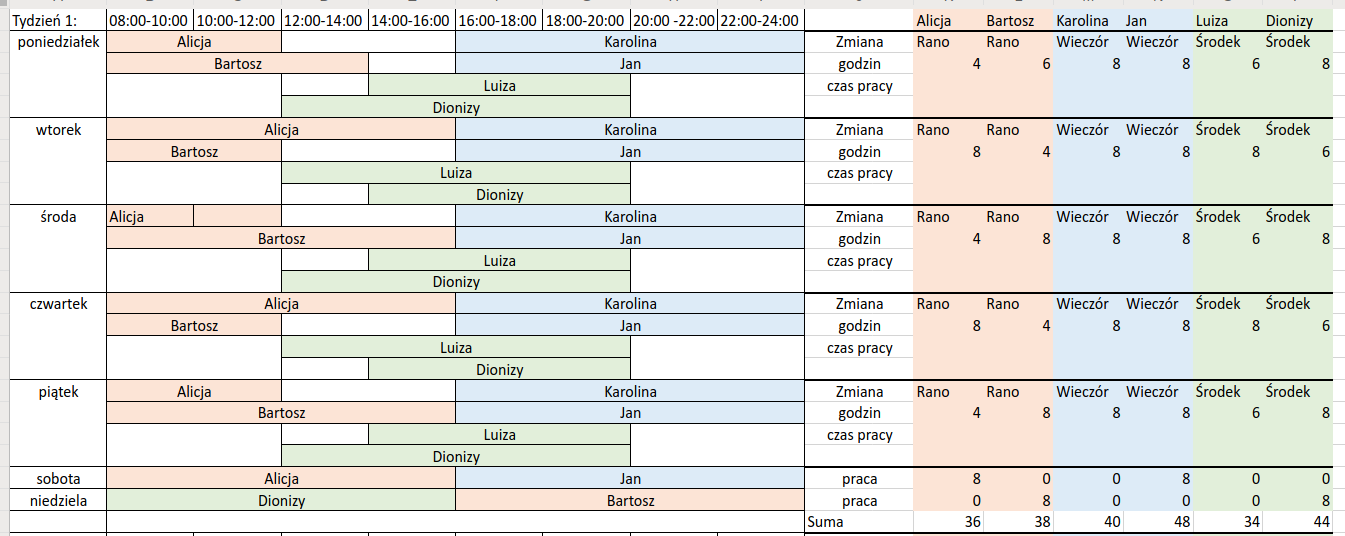
\includegraphics[scale=.48, angle =  90]{93547771_2313519675615944_2694907324711043072_n.png} 

\end{center}


\end{document}